\documentclass[spanish]{udpreport}
\usepackage[utf8]{inputenc}
\usepackage[spanish]{babel}

% Podemos establecer el logo de alguna entidad o dejar el de la UDP (defecto)
%\setlogo{EITFI}

\title{Informe de redes de datos 6\\
"Enrutamiento"\\}
\author{Alumno: Camilo Araya
\\Profesor: Nicolás Hidalgo\\Ayudante: Martín Griño}
\date{\today}



\begin{document}
\maketitle

\chapter*{Resumen} 
\addcontentsline{toc}{section}{Resumen} 
\markboth{RESUMEN}{RESUMEN} 
El presente informe tiene por objetivo trabajar con dos protocolos de ruteo dinámico visto durante el laboratorio los cuales serán EIGRP y OSPF, estos se pondrán en practica en el simulador Cisco Packet Tracer el cual mediante los comandos entregados por el ayudante se podrán configurar ambos protocolos con el fin de discriminar su funcionamiento y eficiencia en el caso planteado en la experiencia de laboratorio.
\tableofcontents
\chapter{Introducción}
La forma en que los router se les de la orden de enrutar es mediante el uso de protocolos, que en resumidas cuentas son ordenes que se les indica para que ejecuten alguna acción correspondiente a el fin que se desea llegar. El objetivo de crear protocolos de enrutamiento es para construir la tabla de enrutamiento de manera automática al hacer uso de dichos protocolos, junto con esto se permite a partir de lo mencionado anteriormente que los routers compartan la información entre ellos lo que hará mas efectivo el envió.
\section{EIGRP}
Es un protocolo de enrutamiento de Gateway interior mejorado, combina las ventajas de los protocolos de estado de enlace con los del vector de distancia, este algoritmo es híbrido ya que se forma a partir de la combinación de los dos protocolos, por otra parte hay que destacar que los routers mediante la formación de adyacencias aprenden dinámicamente rutas nuevas que unen a la red. Este protocolo fue implementado por Cisco.
\begin{figure}[h]
    \centering
    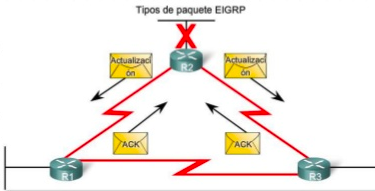
\includegraphics[scale=0.3]{images/ei.png}
    \caption{Topología}
    \label{fig:my_label}
\end{figure}
\section{OSPF}
Es un protocolo de ruteo interno basado en estado enlace, es decir, en vez de procesar los caminos basándose en el vector distancia, mantienen un mapa de la topología de red la cual nos ofrece una visión mas global de esta misma. Este protocolo es Open Source, es decir que todos los aparatos pueden implementarlo y no necesariamente cisco, ha sido pensado para el entorno de internet. Este protocolo fue implementado por IETF.
\begin{figure}[h]
    \centering
    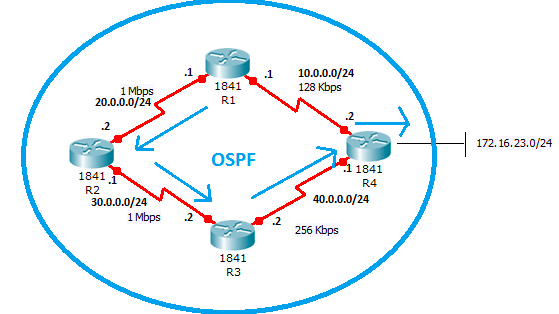
\includegraphics[scale=0.3]{images/osp.png}
    \caption{Topología}
    \label{fig:my_label}
\end{figure}
\chapter{Desarrollo practico}
\section{Primera Actividad}
En esta primera parte del desarrollo práctico se implementara una topología de tres router y se implementara el protocolo EIRGP.\\
\begin{figure}[h]
    \centering
    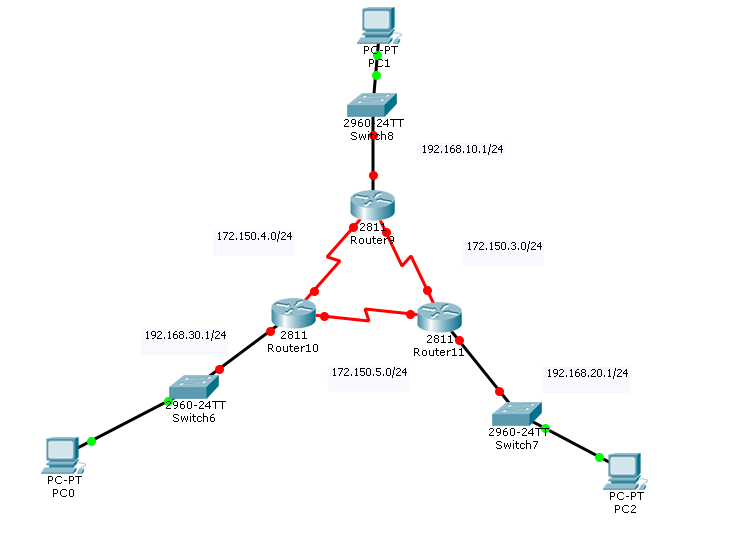
\includegraphics[scale=0.4]{images/11.png}
    \caption{Topología}
    \label{fig:my_label}
\end{figure}
\\
Para poder configurar cada router se aplica los siguientes comandos tomando como referencia el router 9 como se puede apreciar en la \textbf{Figura 2.1}.Cabe destacar que el comando explicado contiene la conexión entre router y LANs.
\begin{figure}[h]
    \centering
    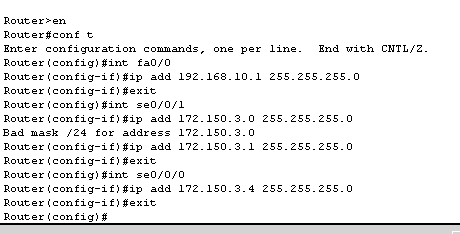
\includegraphics[scale=0.4]{images/22.png}
    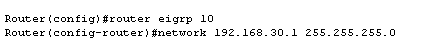
\includegraphics[scale=0.5]{images/112.png}
    \caption{Comandos}
    \label{fig:my_label}
\end{figure}
\\ Estos comandos me permiten realizar ala configuración del protocolo EIGRP el cual como se menciono en la introduccion funciona con un algoritmo hibrido
\section{Segunda Actividad}
Para esta actividad y según lo proporcionado por el ayudante, se realiza el mismo proceso, es decir, aplicar el protocolo EIGRP pero realizado para otro tipo de topología, la cual contendrá 4 router, esta se detallara a continuación.
\begin{figure}[h]
    \centering
    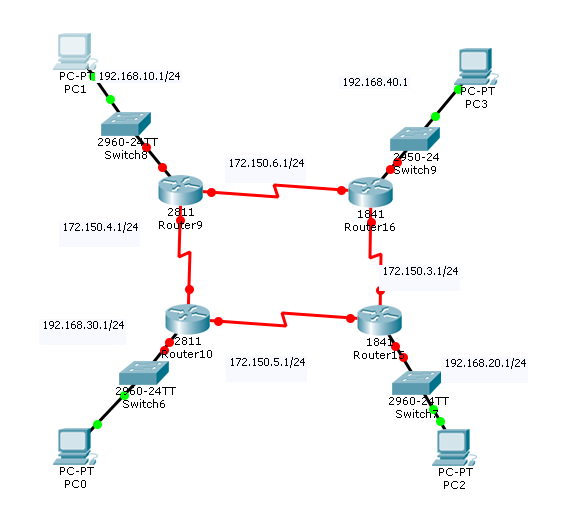
\includegraphics[scale=0.4]{images/co.png}
    \caption{Topología}
    \label{fig:my_label}
\end{figure}
\\ Aquí, al igual que en la parte anterior, se ejecutan los mismos comandos proporcionados por el ayudante, los cuales para efectos prácticos resultara ser lo mismo. 
\\
\begin{figure}[h]
    \centering
    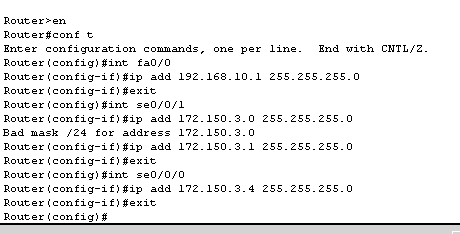
\includegraphics[scale=0.4]{images/22.png}
    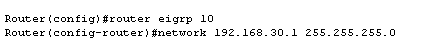
\includegraphics[scale=0.5]{images/112.png}
    \caption{Comandos}
    \label{fig:my_label}
\end{figure}
\chapter{Cuestionario}
\begin{enumerate}
    \item ¿Cual es la diferencia entre los algoritmos de Dijkstra y Bellman Ford?\\
    El algoritmo Bellman Ford solo utiliza la información de sus vecinos y el conocimiento de sus costos de enlace los cuales le serán de utilidad al momento de actualizar sus costos y rutas. Por otro lado, el algoritmo Dijkstra requiere que cada nodo contenga la información topologica completa de la red, es decir, cada nodo sabe los costos de vincular los enlaces en la red.
    \item Mencione dos protocolos de ruteo de cada algoritmo (Dijkstra y Bellman Ford)\\
    Para el algoritmo Bellman Ford se tiene el protocolo RIP y IGRP. Para el algoritmo de Dijkstra los protocolos son OSPF y EIGRP (este ultimo tiene ambos algoritmos.)
    \item ¿Que es más eficiente IGRP u OSPF? por que?\\
    IGRP es un protocolo de vector distancia y OSPF es un protocolo de estado enlace. IGRP sufre ineficiencia con el ancho de banda ya que envían periódicamente sus tablas de enrutamiento y la velocidad de convergencia no es muy buena, es por ello que OSPF es más eficiente ya que mantiene una vista de la topología de red completa y solo emite actualizaciones en su tabla, esto hace que ahorre mucho ancho de banda.
    \item ¿En que caso usaría vector distancia y en cual estado de enlace?\\
    El protocolo estado enlace (utilizado en el protocolo OSPF) se adapta bien a los cambios de topología en la red y es bueno para redes grandes, mientras que el protocolo vector distancia (utilizado por protocolo RIP)le cuesta mas adaptarse al cambio, es por ello que al poder almacenar distancias es mas conveniente utilizarlo para redes que no tengan loops en su topología o bien cuando se agregue un nuevo nodo, este al funcionar por 'rumor' obtendrá su distancia hasta el.
    \item ¿Que algoritmo tiene menor tiempo de convergencia si se agrega un nuevo equipo a la red?\\
    El algoritmo que utilizan los protocolos de ruteo que tiene menor tiempo de convergencia al agregar un nuevo nodo es Dijkstra ya que no cuenta con un conteo de saltos lo cual lo hará mas eficiente.
    
\end{enumerate}
\chapter{Conclusión}
Del presente informe se concluye que el trabajo con ruteo dinámico fue interesante para adentrarse en los tipos de protocolos que se pueden utilizar para una red dependiendo de las utilidades que se implementen. \\Los protocolos utilizados para ruteo dinámico como EIGRP y OSPF no tienen un funcionamiento azaroso, es decir, que se basa en una serie algoritmos los cuales tienen la finalidad tomar las rutas mas óptimas. \\En el trabajo practico se implementaron ambos protocolos con la finalidad de analizar el funcionamiento y a su vez discriminar cual es mejor para los requerimientos establecidos para esta experiencia de laboratorio. Cabe destacar que a pesar se seguir todos los pasos correspondientes los objetivos del laboratorio en si quedaron incompletos debido a que no se alcanzo a ver en la experiencia la configuración del protocolo OSPF.
\begin{thebibliography}{0}
\bibitem{1}Configuración de EIGRP. Recuperado de: \\ \url{http://aprenderedes.com/2006/10/configuracion-de-eigrp/}
\bibitem{2}OSPF, que es? que funcionamiento tiene?. Recuperado de: \\
\url{https://netjnl.wordpress.com/2013/08/28/ospf-que-es-por-que-ospf-mensajes-ospf/}
\end{thebibliography}
\listoffigures
\end{document}

